\documentclass[border=3pt]{standalone}
\usepackage[utf8]{inputenc}
\usepackage[T1]{fontenc}
\usepackage{lmodern}
\renewcommand{\familydefault}{\sfdefault}
\usepackage{sansmath}\sansmath
\usepackage{chemfig}
\usepackage{pgfplots}\pgfplotsset{compat=1.18,/pgf/number format/use comma,/pgf/number format/1000 sep={.}}
\usetikzlibrary{arrows.meta,calc,positioning,decorations.pathmorphing,patterns}
% paleta del sitio
\definecolor{nar}{HTML}{E8680C}\definecolor{narc}{HTML}{FFB35C}\definecolor{hielo}{HTML}{FFF3E8}
\definecolor{tinta}{HTML}{1D1D1F}\definecolor{gris}{HTML}{6E6E73}\definecolor{lila}{HTML}{7C5CF0}
\definecolor{azul}{HTML}{2F6FD6}\definecolor{menta}{HTML}{17A673}\definecolor{coral}{HTML}{E8342A}
\setchemfig{atom sep=2em,bond style={line width=0.8pt}}
\tikzset{lab/.style={font=\small\bfseries,text=nar},pie/.style={font=\footnotesize,text=tinta,align=center}}
\begin{document}
\scalebox{0.7}{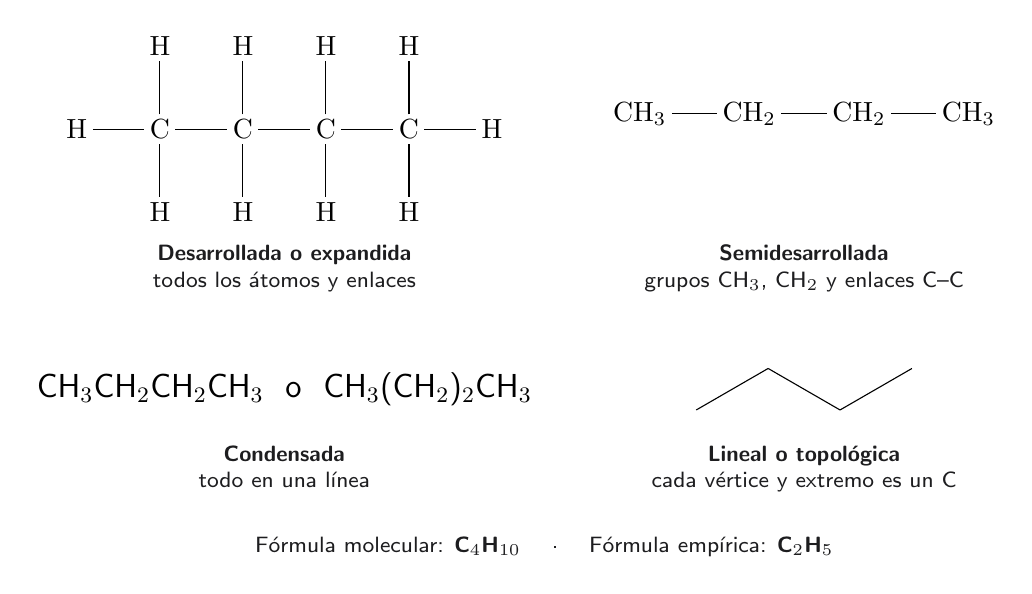
\begin{tikzpicture}
\node (a) at (0,0) {\chemfig{H-C(-[2]H)(-[6]H)-C(-[2]H)(-[6]H)-C(-[2]H)(-[6]H)-C(-[2]H)(-[6]H)-H}};
\node[pie,anchor=north] at (0,-1.35) {\textbf{Desarrollada o expandida}\\todos los átomos y enlaces};
\node at (6.6,0.2) {\chemfig{CH_3-CH_2-CH_2-CH_3}};
\node[pie,anchor=north] at (6.6,-1.35) {\textbf{Semidesarrollada}\\grupos CH$_3$, CH$_2$ y enlaces C--C};
\node at (0,-3.3) {\large CH$_3$CH$_2$CH$_2$CH$_3$ \ o \ CH$_3$(CH$_2$)$_2$CH$_3$};
\node[pie,anchor=north] at (0,-3.9) {\textbf{Condensada}\\todo en una línea};
\node at (6.6,-3.3) {\chemfig{-[:30]-[:-30]-[:30]}};
\node[pie,anchor=north] at (6.6,-3.9) {\textbf{Lineal o topológica}\\cada vértice y extremo es un C};
\node[pie] at (3.3,-5.3) {Fórmula molecular: \textbf{C$_4$H$_{10}$} \quad · \quad Fórmula empírica: \textbf{C$_2$H$_5$}};
\end{tikzpicture}}
\end{document}
